\documentclass[11pt]{article}
\usepackage[T1]{fontenc}
\usepackage[utf8]{inputenc}
\usepackage{lmodern}
\usepackage[final]{microtype}
\usepackage[a4paper,margin=29mm,headheight=15pt]{geometry}
\usepackage{amsmath,amssymb,amsthm,mathtools}
\usepackage{booktabs,longtable,array}
\usepackage{enumitem}
\usepackage{xcolor}
\usepackage{fancyhdr}
\usepackage{hyperref}
\usepackage[nameinlink,noabbrev]{cleveref}
\usepackage{listings}
\usepackage{url}
\usepackage{tikz}
\usetikzlibrary{arrows.meta,positioning}
\definecolor{accent}{HTML}{315B8A}
\definecolor{soft}{HTML}{EEF3F8}
\definecolor{linkblue}{HTML}{1F5A94}
\hypersetup{colorlinks=true,linkcolor=linkblue,citecolor=linkblue,urlcolor=linkblue,
 pdftitle={The Fabius Function and Rvachev's Up Function},
 pdfauthor={OpenAI, guided by Vladimir Reshetnikov's Lean formalization}}
\pagestyle{fancy}\fancyhf{}
\fancyhead[L]{\small\textsc{Fabius and Rvachev's Up Function}}
\fancyhead[R]{\small\nouppercase{\leftmark}}\fancyfoot[C]{\thepage}
\setlength{\parindent}{1.2em}\setlength{\parskip}{0.22em}
\setlist{itemsep=0.2em,topsep=0.45em}\allowdisplaybreaks[2]
\newtheorem{theorem}{Theorem}[section]
\newtheorem{proposition}[theorem]{Proposition}
\newtheorem{lemma}[theorem]{Lemma}
\newtheorem{corollary}[theorem]{Corollary}
\newtheorem{conjecture}[theorem]{Conjecture}
\theoremstyle{definition}
\newtheorem{definition}[theorem]{Definition}
\newtheorem{algorithm}[theorem]{Algorithm}
\newtheorem{example}[theorem]{Example}
\theoremstyle{remark}
\newtheorem{remark}[theorem]{Remark}
\newtheorem{warning}[theorem]{Warning}
\newcommand{\R}{\mathbb R}\newcommand{\C}{\mathbb C}\newcommand{\Z}{\mathbb Z}
\newcommand{\N}{\mathbb N}\newcommand{\Q}{\mathbb Q}
\newcommand{\E}{\mathbb E}\newcommand{\Prob}{\mathbb P}
\newcommand{\Var}{\operatorname{Var}}\newcommand{\supp}{\operatorname{supp}}
\newcommand{\wt}{\operatorname{wt}_2}\newcommand{\upfun}{\operatorname{up}}
\newcommand{\dd}{\,\mathrm d}\newcommand{\e}{\mathrm e}\newcommand{\ii}{\mathrm i}
\newcommand{\ind}{\mathbf 1}\newcommand{\floor}[1]{\left\lfloor#1\right\rfloor}
\newcommand{\abs}[1]{\left|#1\right|}\newcommand{\norm}[1]{\left\|#1\right\|}
\lstset{basicstyle=\ttfamily\small,columns=fullflexible,frame=single,
 rulecolor=\color{accent},backgroundcolor=\color{soft},breaklines=true,showstringspaces=false}
\title{\vspace{-1.3cm}\textbf{The Fabius Function and Rvachev's Up Function}\\[0.4em]
\large Probability, Fourier Analysis, Dyadic Arithmetic, and the Corrected Endpoint Asymptotic}
\author{A human-readable development guided by the Lean~4 formalization\\
\small in \texttt{VladimirReshetnikov/ProveIt}}
\date{24 August 2026}
\begin{document}
\maketitle
\begin{abstract}
The Fabius function is a strictly increasing, infinitely differentiable, nowhere analytic distribution function on the unit interval.  Its twin, Rvachev's \emph{up function}, is an even nonnegative compactly supported bump whose derivative is the difference of two translated and rescaled copies of itself.  These deceptively simple functions connect probability, infinite convolutions, refinable functions, Fourier products, the Thue--Morse sequence, rational arithmetic, $2$-adic valuations, Legendre expansions, the Gamma and zeta functions, Lambert $W$, and saddle-point analysis.

This article presents the principal theorem-level content of the Lean development in the \texttt{ProveIt} repository in conventional mathematical language, with proofs.  It distinguishes carefully among the bounded cumulative distribution function $F$, its signed global self-differential extension $\Theta$, and the compactly supported up function $u$.  Particular emphasis is placed on two topics.  First, every dyadic value $F(a/2^n)$ is evaluated by an explicit finite Thue--Morse/moment formula and by an exact Taylor recursion that clears one nonzero binary digit per step; denominator bounds and the exact valuation
\[
 \nu_2(F(2^{-n}))=-\binom n2-\nu_2(n!)-1
\]
are proved.  Second, the endpoint asymptotic is developed from an exact dyadic decomposition of the negative Laplace transform.  If $L=\log2$ and $\lambda 2^{-\lambda}=x$, then
\[
 \log F(x)=-\frac L2\lambda^2+\left(1+\frac L2\right)\lambda
 -\frac12\log\lambda+C+\Psi(\lambda)+O(\lambda^{-1}),
\]
where $\Psi$ is a nonconstant one-periodic function with explicit Gamma--zeta Fourier coefficients.  Omitting $\Psi$ makes the often quoted $O(1/(-\log x))$ remainder false.  An all-orders exact-Lambert expansion and its first correction are also given.
\end{abstract}
\begin{center}\begin{minipage}{0.93\textwidth}\small
\textbf{Notation warning.}  Some sources use the same symbol for two different functions.  Here $F$ is the bounded CDF, extended constantly outside $[0,1]$; $\Theta$ is the signed global solution of $\Theta'(x)=2\Theta(2x)$; and $u=\upfun$ is Rvachev's compactly supported bump.
\end{minipage}\end{center}
\tableofcontents\newpage

\section{The three related functions}
\subsection{History and scope}
The compactly supported density appeared through its Fourier transform in work of Jessen and Wintner in 1935.  Fabius used the associated distribution function in 1966 as a probabilistic example of a nowhere analytic $C^\infty$ function.  Rvachev rediscovered the bump from the differential--difference equation
\[
 y'(t)=2\bigl(y(2t+1)-y(2t-1)\bigr),
\]
and Arias de Reyna subsequently developed its analysis and arithmetic \cite{JessenWintner,Fabius1966,RvachevBook,Arias1982,AriasArithmetic}.  The Lean formalization underlying this article separates the different objects that were sometimes conflated in the literature and verifies both classical papers, exact dyadic algorithms, a Fourier--Legendre expansion, and a corrected endpoint asymptotic \cite{ReshetnikovLean,ReshetnikovAudit}.

\begin{center}
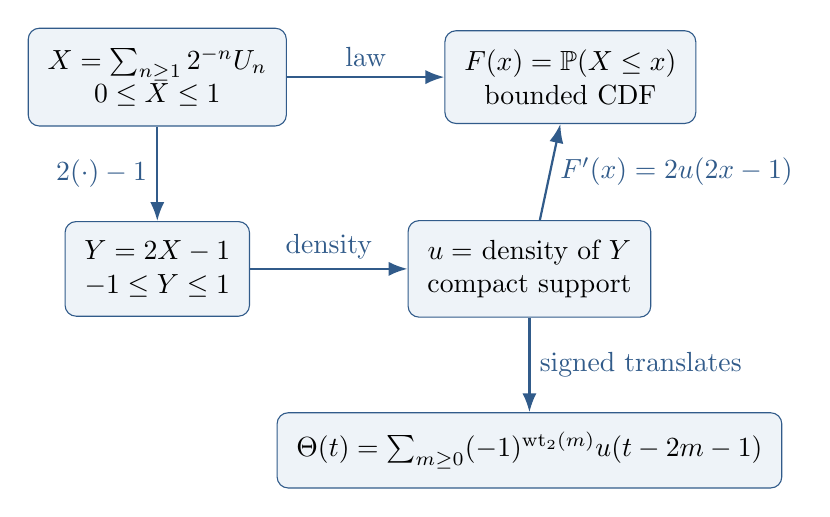
\begin{tikzpicture}[node distance=12mm and 20mm,
box/.style={draw=accent,rounded corners,fill=soft,inner sep=7pt,align=center},
arr/.style={-{Latex[length=2.4mm]},thick,color=accent}]
\node[box] (X) {$X=\sum_{n\ge1}2^{-n}U_n$\\$0\le X\le1$};
\node[box,right=of X] (F) {$F(x)=\Prob(X\le x)$\\bounded CDF};
\node[box,below=of X] (Y) {$Y=2X-1$\\$-1\le Y\le1$};
\node[box,right=of Y] (u) {$u=$ density of $Y$\\compact support};
\node[box,below=of u] (T) {$\Theta(t)=\sum_{m\ge0}(-1)^{\wt(m)}u(t-2m-1)$};
\draw[arr] (X)--node[above]{law}(F);
\draw[arr] (X)--node[left]{$2(\cdot)-1$}(Y);
\draw[arr] (Y)--node[above]{density}(u);
\draw[arr] (u)--node[right]{signed translates}(T);
\draw[arr] (u)--node[right]{$F'(x)=2u(2x-1)$}(F);
\end{tikzpicture}
\end{center}

\subsection{Probability construction}
Let $U_1,U_2,\ldots$ be independent and uniform on $[0,1]$, and put
\begin{equation}\label{eq:X}
 X=\sum_{n=1}^{\infty}2^{-n}U_n,
 \qquad F(x)=\Prob(X\le x).
\end{equation}
The series converges absolutely for every outcome and takes values in $[0,1]$.  We extend $F$ by $0$ on $(-\infty,0]$ and by $1$ on $[1,\infty)$.

\begin{proposition}\label{prop:symmetrymoments}
For $0\le x\le1$,
\[
 F(1-x)=1-F(x),
 \qquad \E X=\frac12,
 \qquad \Var(X)=\frac1{36}.
\]
\end{proposition}
\begin{proof}
The variables $1-U_n$ are again independent uniforms, and
$1-X=\sum 2^{-n}(1-U_n)$, so $X$ and $1-X$ have the same law.  The law will be shown to have a continuous density, giving the symmetry formula without endpoint atoms.  Linearity and independence give
\[
 \E X=\sum_{n\ge1}2^{-n}\frac12=\frac12,
 \qquad
 \Var(X)=\sum_{n\ge1}4^{-n}\frac1{12}=\frac1{36}.
\]
\end{proof}

Set $V_n=2U_n-1$, so the $V_n$ are independent uniforms on $[-1,1]$, and
\begin{equation}\label{eq:Y}
 Y=2X-1=\sum_{n=1}^{\infty}2^{-n}V_n.
\end{equation}
The density of $Y$ is Rvachev's up function $u$.  Thus
\begin{equation}\label{eq:F-u-density}
 F'(x)=2u(2x-1),
 \qquad
 F(x)=\int_{-1}^{2x-1}u(t)\dd t.
\end{equation}
On the support, the two functions are related without differentiation:
\begin{equation}\label{eq:u-from-F}
 u(t)=\begin{cases}
 F(t+1),&-1\le t\le0,\\
 F(1-t),&0\le t\le1,\\
 0,&|t|>1.
 \end{cases}
\end{equation}

\section{Existence and uniqueness of the up function}\label{sec:existence}
Use the Fourier convention
\begin{equation}\label{eq:fourier-convention}
 \widehat f(z)=\int_{\R}f(t)\e^{-2\pi\ii zt}\dd t.
\end{equation}
Suppose $v\in C_c^\infty(\R)$ is supported on $[-1,1]$, positive on the interior, $v(0)=1$, and
\begin{equation}\label{eq:general-up}
 v'(t)=k\bigl(v(2t+1)-v(2t-1)\bigr),\qquad k>0.
\end{equation}
Fourier transformation gives
\begin{equation}\label{eq:fourier-scale-general}
 \widehat v(z)=\frac{k}{2}\frac{\sin\pi z}{\pi z}\widehat v(z/2).
\end{equation}

\begin{theorem}[Rvachev's characterization]\label{thm:up-existence}
There is a unique $u\in C_c^\infty(\R)$ such that $\supp u=[-1,1]$, $u>0$ on $(-1,1)$, $u(0)=1$, and \eqref{eq:general-up} holds for some positive $k$.  Necessarily $k=2$.  The function is even, nonnegative, and normalized by $\int u=1$.
\end{theorem}
\begin{proof}
Iterating \eqref{eq:fourier-scale-general} gives
\[
 \widehat v(z)=\left(\frac{k}{2}\right)^{N+1}
 \prod_{j=0}^{N}\frac{\sin(\pi z/2^j)}{\pi z/2^j}
 \widehat v(z/2^{N+1}).
\]
At $z=0$, positivity gives $\widehat v(0)>0$, hence $k=2$.  Letting $N\to\infty$ yields
\begin{equation}\label{eq:up-product}
 \widehat v(z)=\widehat v(0)
 \prod_{j=0}^{\infty}\frac{\sin(\pi z/2^j)}{\pi z/2^j}.
\end{equation}
Fourier inversion determines $v$ up to the scalar $\widehat v(0)$, and $v(0)=1$ fixes the scalar.  This proves uniqueness.

For existence define the product with scalar $1$.  On compact subsets of $\C$, its factors are $1+O(4^{-j}|z|^2)$, so it converges locally uniformly.  On the real line, taking any fixed number of initial factors and bounding their numerators by $1$ shows decay faster than every inverse power.  Its inverse Fourier transform $u$ is therefore $C^\infty$, and the scale identity transforms back to
\begin{equation}\label{eq:up-dde}
 u'(t)=2\bigl(u(2t+1)-u(2t-1)\bigr).
\end{equation}

To obtain support and positivity without invoking Paley--Wiener, use
\[
 \frac{\sin z}{z}=\prod_{m=1}^{\infty}\cos(z/2^m)
\]
to rewrite the transform as $\prod_{m\ge1}(\cos(\pi z/2^m))^m$.  The $M$th truncation is the Fourier transform of a finite convolution of symmetric two-point probability measures
\[
 \frac12\delta_{2^{-m-1}}+\frac12\delta_{-2^{-m-1}},
\]
with the $m$th measure repeated $m$ times.  The total support radius is at most
$\sum_{m\ge1}m/2^{m+1}=1$.  Weak compactness and uniqueness of Fourier transforms show that the truncations converge to the probability measure $u(t)\dd t$, supported on $[-1,1]$.  Hence $u\ge0$ and $\int u=1$.

For $-1<x<0$, integrating \eqref{eq:up-dde} from $-1$ to $x$ gives
\begin{equation}\label{eq:positive-propagation}
 u(x)=2\int_{-1}^{x}u(2t+1)\dd t.
\end{equation}
Nonnegativity and nonzero mass propagate strict positivity through $(-1,0)$; symmetry gives it on $(0,1)$.  Finally
\[
 u(0)=\int_{-1}^{0}u'(t)\dd t
 =2\int_{-1}^{0}u(2t+1)\dd t=\int_{-1}^{1}u(s)\dd s=1.
\]
\end{proof}

\subsection{Infinite convolution descriptions}
The density of $2^{-n}V_n$ is $2^{n-1}\ind_{[-2^{-n},2^{-n}]}$, so
\begin{equation}\label{eq:uniform-convolution}
 u=\mathop{*}_{n=1}^{\infty}
 \left(2^{n-1}\ind_{[-2^{-n},2^{-n}]}\right).
\end{equation}
This immediately reproduces the sine product.  The Bernoulli convolution in the proof gives a second model: if $\varepsilon_{m,j}$ are independent symmetric signs, then
\[
 \sum_{m=1}^{\infty}\sum_{j=1}^{m}2^{-m-1}\varepsilon_{m,j}
\]
has density $u$.  The first model is best for probability; the second is best for finite combinatorial approximants.

\section{Finite approximants and restricted partitions}\label{sec:approximants}
For $m\ge1$ define
\begin{equation}\label{eq:partition-polynomial}
 p_m(x)=\prod_{j=1}^{m}(1+x+\cdots+x^{2^j-1})
 =\sum_r a_{m,r}x^r.
\end{equation}
The coefficient $a_{m,r}$ counts tuples $(s_1,\ldots,s_m)$ with
$0\le s_j\le2^j-1$ and $s_1+\cdots+s_m=r$.  The recursion
\[
 p_{m+1}(x)=p_m(x)(1+x+\cdots+x^{2^{m+1}-1})
\]
therefore becomes a sliding-window sum for the coefficients.

\begin{proposition}[Step approximants]\label{prop:step-approximants}
There exist even compactly supported step functions $u_m$ whose plateau heights are normalized coefficients of $p_m$, such that $u_m(0)=1$, $\int u_m=1$, $u_m$ increases on $(-1,0)$ and decreases on $(0,1)$, and $u_m(t)\to u(t)$ pointwise when shared jump endpoints are given half weight.  The measures $u_m(t)\dd t$ converge weakly to $u(t)\dd t$.
\end{proposition}
\begin{proof}
Take finite stages of the Bernoulli convolution and group equal atoms.  Their multiplicities are exactly the coefficients of \eqref{eq:partition-polynomial}; integrating the atomic distribution over a cell gives the step functions.  Coefficient symmetry gives evenness, and convolution with a uniform discrete block preserves unimodality.  The characteristic functions converge pointwise to $\widehat u$, all supports remain in $[-1,1]$, and therefore the measures converge weakly to $u(t)\dd t$.  Continuity of the limit and monotonicity of the approximants turn convergence of interval masses into pointwise convergence.  Half weights avoid double counting a shared endpoint.
\end{proof}

\begin{remark}
The endpoint convention is not cosmetic.  A formula using closed cells at both ends counts boundary atoms twice.  The Lean development isolates the half-endpoint statement explicitly.
\end{remark}

\section{The bounded Fabius function}\label{sec:bounded}
\begin{theorem}[Basic identities]\label{thm:F-basic}
The bounded $F$ is $C^\infty$ on $\R$, strictly increasing on $[0,1]$, and
\begin{align}
 F'(x)&=2u(2x-1),&&0\le x\le1,\label{eq:Fprime-u}\\
 F'(x)&=2F(2x),&&0\le x\le\tfrac12,\label{eq:Fprime-left}\\
 F'(x)&=2F(2-2x),&&\tfrac12\le x\le1.\label{eq:Fprime-right}
\end{align}
Moreover
\begin{align}
 F(1-x)&=1-F(x),&F'(1-x)&=F'(x),\label{eq:F-symmetries}\\
 F^{(r)}(0)&=F^{(r)}(1)=0&& (r\ge1),\label{eq:F-flat}
\end{align}
and $F(1/2)=1/2$.
\end{theorem}
\begin{proof}
Equation \eqref{eq:F-u-density} proves smoothness because $u$ is smooth and flat at the endpoints of its support.  On $0\le x\le1/2$, \eqref{eq:u-from-F} gives $u(2x-1)=F(2x)$; on the other half, evenness gives $u(2x-1)=F(2-2x)$.  Positivity of $u$ on the interior makes $F'$ positive.  The symmetry was proved probabilistically, and differentiation gives the derivative symmetry.  Compact support and smoothness of $u$ imply all positive-order derivatives of $F$ vanish at $0$ and $1$.
\end{proof}

\begin{warning}
The equation $F'(x)=2F(2x)$ is valid for the bounded CDF only on $[0,1/2]$.  Its global version belongs to the signed extension $\Theta$ introduced next.
\end{warning}

\section{The signed global extension and the Thue--Morse sequence}\label{sec:theta}
Let $\wt(m)$ denote the number of $1$'s in the binary expansion of $m$.  Thus
\begin{equation}\label{eq:wt-rec}
 \wt(2m)=\wt(m),\qquad \wt(2m+1)=\wt(m)+1.
\end{equation}
Define the locally finite sum
\begin{equation}\label{eq:theta-def}
 \Theta(t)=\sum_{m=0}^{\infty}(-1)^{\wt(m)}u(t-2m-1).
\end{equation}

\begin{theorem}[Global self-differential extension]\label{thm:theta}
The function $\Theta$ is smooth, vanishes for $t\le0$, agrees with $F$ on $[0,1]$, and on $2m\le t\le2m+2$ satisfies
\begin{equation}\label{eq:theta-piece}
 \Theta(t)=(-1)^{\wt(m)}u(t-2m-1).
\end{equation}
Furthermore
\begin{align}
 \Theta'(t)&=2\Theta(2t),\label{eq:theta-prime}\\
 \Theta^{(r)}(t)&=2^{\binom{r+1}{2}}\Theta(2^rt),\qquad r\ge0.\label{eq:theta-derivatives}
\end{align}
At nonnegative integers,
\[
 \Theta(2m)=0,
 \qquad
 \Theta(2m+1)=(-1)^{\wt(m)}.
\]
\end{theorem}
\begin{proof}
Local finiteness and the infinite-order vanishing of $u$ at the endpoints of each translated support give smoothness.  Differentiate \eqref{eq:theta-def} and use \eqref{eq:up-dde}:
\begin{align*}
 \Theta'(t)
 &=2\sum_{m\ge0}(-1)^{\wt(m)}
 \{u(2t-4m-1)-u(2t-4m-3)\}\\
 &=2\sum_{m\ge0}(-1)^{\wt(2m)}u(2t-2(2m)-1)
  +2\sum_{m\ge0}(-1)^{\wt(2m+1)}u(2t-2(2m+1)-1)\\
 &=2\Theta(2t),
\end{align*}
where \eqref{eq:wt-rec} supplies the second sign.  Induction then yields \eqref{eq:theta-derivatives}.  The support description gives \eqref{eq:theta-piece}, agreement with $F$ on $[0,1]$, and the integer values.
\end{proof}

\begin{corollary}[All derivatives from one global function]\label{cor:u-derivatives}
For $-1\le t\le1$ and $r\ge0$,
\begin{equation}\label{eq:u-derivatives}
 u^{(r)}(t)=2^{\binom{r+1}{2}}
 \Theta(2^rt+2^r).
\end{equation}
\end{corollary}
\begin{proof}
On $[-1,1]$, $u(t)=\Theta(t+1)$.  Differentiate and apply \eqref{eq:theta-derivatives}.
\end{proof}

\subsection{Nowhere analyticity}
\begin{theorem}[Exact dyadic jets]\label{thm:dyadic-jets}
Let $t=q/2^n\in(-1,1)$ be reduced, so $q$ is odd when $n>0$.  Then
\[
 u^{(r)}(t)=0\quad(r>n),
 \qquad
 u^{(n)}(t)\ne0.
\]
The Taylor series at $t$ is therefore a polynomial of exact degree $n$.
\end{theorem}
\begin{proof}
For $r>n$, the argument in \eqref{eq:u-derivatives} is
$2^{r-n}q+2^r$, an even integer, where $\Theta$ vanishes.  At $r=n$ the argument is the odd integer $q+2^n$, where $\Theta=\pm1$.  Hence
$u^{(n)}(t)=\pm2^{\binom{n+1}{2}}$.
\end{proof}

\begin{corollary}\label{cor:nowhere-analytic}
Neither $u$ on $[-1,1]$ nor $F$ on $[0,1]$ is real analytic at any point.
\end{corollary}
\begin{proof}
At every dyadic point the Taylor series is a finite polynomial, but the function cannot agree with it on a neighborhood: a sufficiently high derivative would then vanish on an interval, contradicting the translated self-similar formula and strict positivity.  Hence $u$ is nonanalytic at every dyadic point.  If it were analytic at any point, it would be analytic on a small interval containing a dyadic point, a contradiction.  The conclusion for $F$ follows from $F'(x)=2u(2x-1)$.
\end{proof}

\section{Fourier analysis and partitions of unity}\label{sec:fourier}
\begin{theorem}[Three Fourier products]\label{thm:fourier-products}
For every $z\in\C$,
\begin{equation}\label{eq:three-products}
\begin{aligned}
 \widehat u(z)
 &=\prod_{n=0}^{\infty}\frac{\sin(\pi z/2^n)}{\pi z/2^n}\\
 &=\prod_{m=1}^{\infty}\left(\cos\frac{\pi z}{2^m}\right)^m\\
 &=\prod_{m=1}^{\infty}
 \left(1-\frac{z^2}{m^2}\right)^{1+\nu_2(m)}.
\end{aligned}
\end{equation}
The products converge locally uniformly.  The nonzero zeros are exactly the integers, and the zero at $m\ne0$ has multiplicity $1+\nu_2(|m|)$.
\end{theorem}
\begin{proof}
The first product is \eqref{eq:up-product} with the normalization $\widehat u(0)=1$.  Apply
$\sin w/w=\prod_{j\ge1}\cos(w/2^j)$ and count pairs $n+j=m$ to obtain the cosine product: a fixed denominator $2^m$ occurs exactly $m$ times.  Finally use
$\sin\pi w/(\pi w)=\prod_{r\ge1}(1-w^2/r^2)$.  The factor indexed by $n$ vanishes at an integer $m$ exactly when $2^n\mid m$, giving the multiplicity count.
\end{proof}

\begin{proposition}[Rapid decay and inversion]\label{prop:rapid-decay}
For every $N$ there is $C_N$ with
\[
 |\widehat u(\xi)|\le C_N(1+|\xi|)^{-N}.
\]
Consequently
\begin{equation}\label{eq:fourier-inversion}
 u^{(r)}(t)=\int_{\R}(2\pi\ii\xi)^r\widehat u(\xi)
 \e^{2\pi\ii\xi t}\dd\xi
\end{equation}
with absolute convergence.
\end{proposition}
\begin{proof}
For large $|\xi|$, bound the numerators of any chosen number of initial sine factors by $1$; those factors contribute the desired inverse power, while every remaining real factor has modulus at most $1$.  Fourier inversion and differentiation under the integral follow.
\end{proof}

\begin{theorem}[Poisson summation]\label{thm:poisson}
For $a>0$,
\begin{equation}\label{eq:poisson}
 \sum_{m\in\Z}u(t+am)=\frac1a\sum_{k\in\Z}
 \widehat u\!\left(\frac{k}{a}\right)\e^{2\pi\ii kt/a}.
\end{equation}
\end{theorem}
\begin{proof}
The left side is a smooth $a$-periodic function.  Its $k$th Fourier coefficient is
\[
 \frac1a\int_0^a\sum_m u(t+am)\e^{-2\pi\ii kt/a}\dd t
 =\frac1a\int_{\R}u(v)\e^{-2\pi\ii kv/a}\dd v
 =\frac1a\widehat u(k/a).
\]
Rapid decay gives absolute convergence of the Fourier series.
\end{proof}

\begin{corollary}[Partitions of unity]\label{cor:partition}
For every positive integer $n$,
\begin{equation}\label{eq:fine-partition}
 \sum_{m\in\Z}u\!\left(t+\frac mn\right)=n.
\end{equation}
In particular $\sum_m u(t+m)=1$, and on $0\le t\le1$,
\begin{equation}\label{eq:two-term-partition}
 u(t)+u(t-1)=1.
\end{equation}
Consequently, for $0\le x\le1/2$,
\[
 F'(x)+F'(1/2-x)=2.
\]
\end{corollary}
\begin{proof}
Set $a=1/n$ in \eqref{eq:poisson}.  Every nonzero Fourier term is $\widehat u(nk)=0$ by \cref{thm:fourier-products}.  Support reduces the integer partition to two terms on $[0,1]$.  Substitute $t=2x$ and use \eqref{eq:Fprime-u} for the last identity.
\end{proof}

\begin{corollary}[Cosine series]\label{cor:cosine}
For $-1\le t\le1$,
\begin{equation}\label{eq:cosine}
 u(t)=\frac12+\sum_{k=0}^{\infty}
 \widehat u\!\left(\frac{2k+1}{2}\right)
 \cos((2k+1)\pi t),
\end{equation}
with absolute and uniform convergence, together with all derivatives.
\end{corollary}
\begin{proof}
Use Poisson summation with period $2$.  Integer frequencies vanish, and pairing opposite half-integer frequencies gives the cosine series.
\end{proof}

\begin{remark}[A source-level correction]
The exponential in Poisson summation must contain the variable $t$: it is $\e^{2\pi\ii kt/a}$.  A printed version of the formula loses this factor.  The Fourier-coefficient computation above makes the correction immediate.
\end{remark}

\section{Moments and generating functions}\label{sec:moments}
Define
\begin{equation}\label{eq:c-def}
 c_n=\int_{-1}^{1}t^{2n}u(t)\dd t.
\end{equation}
Then
\begin{equation}\label{eq:fourier-moment-series}
 \widehat u(z)=\sum_{n=0}^{\infty}(-1)^n
 \frac{c_n}{(2n)!}(2\pi z)^{2n}.
\end{equation}

\begin{theorem}[Even-moment recurrence]\label{thm:c-recurrence}
The positive rational numbers $c_n$ are determined by
\begin{equation}\label{eq:c-recurrence}
 c_0=1,
 \qquad
 (2n+1)(2^{2n}-1)c_n
 =\sum_{k=0}^{n-1}\binom{2n+1}{2k}c_k.
\end{equation}
In particular
\[
 c_0=1,
 \quad c_1=\frac19,
 \quad c_2=\frac{19}{675},
 \quad c_3=\frac{583}{59535},
 \quad c_4=\frac{132809}{32531625}.
\]
\end{theorem}
\begin{proof}
Integrate \eqref{eq:up-dde} against $t^{2n+1}$.  Integration by parts and the substitutions $s=2t\pm1$ give
\[
 (2n+1)2^{2n}c_n=\sum_{k=0}^{n}\binom{2n+1}{2k}c_k.
\]
The final term is $(2n+1)c_n$; move it to the left.  Induction proves rationality and positivity.
\end{proof}

Define the entire function
\begin{equation}\label{eq:G-def}
 \begin{aligned}
 G(z)&=1+z\int_0^1u(t)\e^{zt}\dd t\\
 &=\e^{z/2}\widehat u\!\left(\frac{\ii z}{4\pi}\right)
 =\sum_{n=0}^{\infty}\frac{d_n}{n!}z^n.
 \end{aligned}
\end{equation}
It is also the moment-generating function $G(z)=\E\e^{zX}$.

\begin{theorem}[Half moments]\label{thm:d-recurrence}
One has
\begin{equation}\label{eq:G-functional}
 G(2z)=\frac{\e^z-1}{z}G(z),
\end{equation}
with the removable value at $z=0$, and
\begin{equation}\label{eq:d-recurrence}
 d_0=1,
 \qquad
 (n+1)(2^n-1)d_n
 =\sum_{k=0}^{n-1}\binom{n+1}{k}d_k.
\end{equation}
Moreover
\begin{align}
 d_n&=n\int_0^1t^{n-1}u(t)\dd t,\label{eq:d-half-moment}\\
 d_n&=2^{-n}\sum_{k=0}^{\floor{n/2}}\binom n{2k}c_k.\label{eq:d-from-c}
\end{align}
The first values are
\[
 1,\quad\frac12,\quad\frac5{18},\quad\frac16,
 \quad\frac{143}{1350},\quad\frac{19}{270},\ldots.
\]
\end{theorem}
\begin{proof}
Substitute the Fourier dilation equation into \eqref{eq:G-def}:
\[
 G(2z)=\e^z\frac{\sin(\ii z/2)}{\ii z/2}
 \widehat u\!\left(\frac{\ii z}{4\pi}\right)
 =\frac{\e^z-1}{z}G(z).
\]
Coefficient comparison gives \eqref{eq:d-recurrence}, and the integral definition gives \eqref{eq:d-half-moment}.  Integrating by parts,
\begin{align*}
 d_n&=-\int_0^1t^nu'(t)\dd t
 =2\int_0^1t^nu(2t-1)\dd t\\
 &=\int_{-1}^{1}\left(\frac{s+1}{2}\right)^nu(s)\dd s.
\end{align*}
Expanding and discarding odd moments gives \eqref{eq:d-from-c}.
\end{proof}

\begin{theorem}[Bridge to inverse powers of two]\label{thm:bridge}
For $n\ge1$,
\begin{equation}\label{eq:bridge}
 d_n=n!\,2^{\binom n2}u(1-2^{-n})
 =n!\,2^{\binom n2}F(2^{-n}).
\end{equation}
Consequently
\begin{equation}\label{eq:c-bridge}
 c_n=2(2n)!\,2^{\binom{2n+1}{2}}F(2^{-2n-1}).
\end{equation}
\end{theorem}
\begin{proof}
Define
\[
 f_r(t)=2^{\binom r2}u\!\left(\frac{t}{2^r}-\frac1{2^r}-\frac1{2^{r-1}}-\cdots-\frac12\right).
\]
The differential--difference equation shows $f_{r+1}'=f_r$ on $[-1,1]$, and all $f_r(-1)=0$.  Repeated integration by parts yields
\[
 \int_0^1t^{n-1}u(t)\dd t=(n-1)!2^{\binom n2}u(1-2^{-n}).
\]
Multiply by $n$ and use \eqref{eq:u-from-F}.  The even-moment formula follows by applying the result at index $2n+1$ and doubling the integral over $[0,1]$.
\end{proof}

\subsection{Integral numerator sequences}
Define
\begin{align}
 \mathcal F_n&=c_n(2n+1)!!\prod_{j=1}^{n}(2^{2j}-1),\label{eq:Fn-def}\\
 \mathcal G_n&=d_n(n+1)!\prod_{j=1}^{n}(2^j-1).\label{eq:Gn-def}
\end{align}

\begin{proposition}\label{prop:FG-integral}
Both sequences consist of positive integers.  They satisfy
\begin{align}
 \mathcal F_n&=\sum_{k=0}^{n-1}\mathcal F_k
 \binom{2n+1}{2k}\frac{(2n-1)!!}{(2k+1)!!}
 \prod_{j=k+1}^{n-1}(2^{2j}-1),\label{eq:Fn-rec}\\
 \mathcal G_n&=\sum_{k=0}^{n-1}\mathcal G_k
 \binom{n+1}{k}\frac{n!}{(k+1)!}
 \prod_{j=k+1}^{n-1}(2^j-1).\label{eq:Gn-rec}
\end{align}
In particular
\begin{equation}\label{eq:F-inverse-Gn}
 F(2^{-n})=
 \frac{2^{-\binom n2}\mathcal G_n}
 {n!(n+1)!\prod_{j=1}^{n}(2^j-1)}.
\end{equation}
\end{proposition}
\begin{proof}
Substitute \eqref{eq:Fn-def} into \eqref{eq:c-recurrence} and clear factors to obtain \eqref{eq:Fn-rec}; every factor is integral, so induction applies.  Do the same with \eqref{eq:Gn-def} and \eqref{eq:d-recurrence}.  Formula \eqref{eq:F-inverse-Gn} follows from \eqref{eq:bridge}.
\end{proof}

\subsection{Bernoulli recurrences}
Let $z/(\e^z-1)=\sum B_mz^m/m!$, with $B_1=-1/2$.
\begin{proposition}\label{prop:Bernoulli}
For $n\ge1$,
\begin{align}
 c_n&=\frac1{2^{2n}-1}\sum_{k=1}^{n}2^{2n-2k}(2^{2k}-2)
 \binom{2n}{2k}B_{2k}c_{n-k},\label{eq:c-Bernoulli}\\
 d_n&=\frac{n2^{n-2}}{2^n-1}d_{n-1}
 -\frac1{2^n-1}\sum_{k=1}^{\floor{n/2}}
 \binom n{2k}2^{n-2k}B_{2k}d_{n-2k}.\label{eq:d-Bernoulli}
\end{align}
\end{proposition}
\begin{proof}
Use
\[
 \frac{\pi z}{\sin\pi z}\widehat u(z)=\widehat u(z/2),
 \qquad
 \frac{z}{\e^z-1}G(2z)=G(z),
\]
together with the Bernoulli expansions of the two prefactors, and compare coefficients.
\end{proof}

\section{Exact evaluation at dyadic rationals}\label{sec:dyadic}
This chapter gives two exact methods \cite{AriasArithmetic,Haugland}.  The first is a closed finite sum involving Thue--Morse signs and the moments $c_k$.  The second is a recursive Taylor identity that clears one nonzero binary digit per step.  The finite formula reveals the global derivative structure; the recursion is normally faster in exact arithmetic.

\subsection{A finite formula for the up function}
\begin{theorem}[Global Thue--Morse/moment formula]\label{thm:global-dyadic}
Let $n\ge0$ and $q\in\Z$ with $-2^n<q<2^n$.  Then
\begin{equation}\label{eq:global-dyadic}
\begin{aligned}
 u\!\left(\frac q{2^n}\right)
 ={}&\frac{2^{-\binom{n+1}{2}}}{n!}
 \sum_{h=0}^{q+2^n-1}(-1)^{\wt(h)}
 \sum_{k=0}^{\floor{n/2}}\binom n{2k}\\
 &\quad\times\bigl(2(q-h)+2^{n+1}-1\bigr)^{n-2k}c_k.
\end{aligned}
\end{equation}
\end{theorem}
\begin{proof}
All derivatives of $u$ vanish at $-1$, so Taylor's theorem with integral remainder gives, for $t=q/2^n$,
\begin{equation}\label{eq:taylor-integral-up}
 u(t)=\frac1{n!}\int_{-1}^{t}(t-x)^nu^{(n+1)}(x)\dd x.
\end{equation}
By \eqref{eq:u-derivatives},
\[
 u^{(n+1)}(x)=2^{\binom{n+2}{2}}
 \Theta(2^{n+1}(1+x)).
\]
Split the interval according to
$2h\le2^{n+1}(1+x)\le2h+2$.  On the $h$th piece,
\[
 \Theta(2^{n+1}(1+x))=(-1)^{\wt(h)}
 u(2^{n+1}(1+x)-2h-1).
\]
With $v=2^{n+1}(1+x)-2h-1$, the piece becomes an integral over $[-1,1]$.  Collecting the scale factors gives
\begin{align*}
 u(t)=\frac{2^{-\binom{n+1}{2}}}{n!}
 \sum_{h=0}^{q+2^n-1}(-1)^{\wt(h)}
 \int_{-1}^{1}
 \bigl(2(q-h)+2^{n+1}-1-v\bigr)^nu(v)\dd v.
\end{align*}
Expand the power.  Odd moments vanish by evenness, and the $2k$th moment is $c_k$, yielding \eqref{eq:global-dyadic}.
\end{proof}

\subsection{The bounded finite formula}
\begin{theorem}[Exact formula for $F(a/2^n)$]\label{thm:bounded-dyadic}
For $n\ge0$ and $0\le a\le2^n$,
\begin{equation}\label{eq:bounded-dyadic}
\boxed{\begin{aligned}
 F\!\left(\frac a{2^n}\right)
 ={}&\frac{2^{-\binom{n+1}{2}}}{n!}
 \sum_{h=0}^{a-1}(-1)^{\wt(h)}
 \sum_{k=0}^{\floor{n/2}}\binom n{2k}\\
 &\quad\times(2a-2h-1)^{n-2k}c_k.
\end{aligned}}
\end{equation}
The outer sum is empty when $a=0$.
\end{theorem}
\begin{proof}
Apply \cref{thm:global-dyadic} to $u(1-a/2^n)$ and use $F(a/2^n)=u(1-a/2^n)$, or equivalently shift $q=a-2^n$ in the global formula and use evenness.  The upper limit becomes $a-1$ and the affine factor simplifies to $2a-2h-1$.
\end{proof}

\begin{corollary}\label{cor:dyadic-rational}
Every dyadic value of $F$ and $u$ is rational.
\end{corollary}
\begin{proof}
All terms in \eqref{eq:bounded-dyadic} and \eqref{eq:global-dyadic} are rational because the moments are rational.
\end{proof}

\subsection{Worked finite-sum examples}
\begin{example}[$F(1/4)$]
Take $n=2$, $a=1$.  Since $c_0=1$ and $c_1=1/9$,
\[
 F(1/4)=\frac{2^{-3}}{2!}
 \left(1+\binom22c_1\right)
 =\frac1{16}\left(1+\frac19\right)=\frac5{72}.
\]
\end{example}

\begin{example}[$F(1/8)$]
With $n=3$, $a=1$,
\[
 F(1/8)=\frac{2^{-6}}{3!}
 \left(1+\binom32c_1\right)
 =\frac1{384}\left(1+\frac13\right)=\frac1{288}.
\]
\end{example}

\begin{example}[$F(3/8)$]
The signs for $h=0,1,2$ are $+,-,-$.  Hence
\begin{align*}
 F(3/8)
 &=\frac1{384}\sum_{h=0}^{2}(-1)^{\wt(h)}
 \left((5-2h)^3+\frac13(5-2h)\right)\\
 &=\frac1{384}\left[\left(125+\frac53\right)
 -(27+1)-\left(1+\frac13\right)\right]
 =\frac{73}{288}.
\end{align*}
Symmetry gives $F(5/8)=215/288$.
\end{example}

\subsection{Taylor reduction and bit clearing}
\begin{lemma}[Reflected integral remainder]\label{lem:reflected-remainder}
Let $x>0$, choose $j\in\Z$ with $2^j\le x<2^{j+1}$, and set $y=x-2^j$.  For $N\ge0$,
\begin{equation}\label{eq:reflected-remainder}
 \int_{2^j}^{x}(x-t)^NF^{(N+1)}(t)\dd t
 =-\int_0^y(y-t)^NF^{(N+1)}(t)\dd t,
\end{equation}
where outside $[0,1]$ the derivative identity is interpreted through the signed extension $\Theta$.
\end{lemma}
\begin{proof}
Scale the left integral by $t=2^j(1+s)$.  Repeated differentiation of $\Theta'(t)=2\Theta(2t)$ transports the derivative from the copy centered at $2^j$ to the copy at the origin.  The Thue--Morse sign across the translated copy is negative.  The Jacobian and the $N$th power cancel the derivative's scale factor, leaving the right side.  Within the bounded interval the same calculation can be written piecewise using \eqref{eq:Fprime-left}, \eqref{eq:Fprime-right}, and symmetry.
\end{proof}

\begin{theorem}[Taylor-reduction identity]\label{thm:taylor-reduction}
Let $0<x\le1$ and let $n\ge0$ be uniquely determined by
$2^{-n}\le x<2^{-n+1}$.  Put $y=x-2^{-n}$.  Then
\begin{equation}\label{eq:taylor-reduction}
\boxed{
 F(x)=-F(y)+\sum_{k=0}^{n}
 2^{\binom{k+1}{2}-\binom{n-k}{2}}
 \frac{d_{n-k}}{(n-k)!}\frac{y^k}{k!}.}
\end{equation}
\end{theorem}
\begin{proof}
Taylor-expand at $2^{-n}$ to order $n$:
\[
 F(x)=\sum_{k=0}^{n}\frac{F^{(k)}(2^{-n})}{k!}y^k
 +\frac1{n!}\int_{2^{-n}}^{x}(x-t)^nF^{(n+1)}(t)\dd t.
\]
By \cref{lem:reflected-remainder}, the remainder is
$-n!^{-1}\int_0^y(y-t)^nF^{(n+1)}(t)\dd t=-F(y)$, because all derivatives of $F$ vanish at $0$.  For $0\le k\le n$,
\[
 F^{(k)}(2^{-n})=2^{\binom{k+1}{2}}F(2^{-(n-k)})
 =2^{\binom{k+1}{2}-\binom{n-k}{2}}
 \frac{d_{n-k}}{(n-k)!},
\]
where the last equality is \eqref{eq:bridge}.  Substitution gives the formula.
\end{proof}

\begin{corollary}[Termination at dyadic inputs]\label{cor:bit-clearing}
If $x=a/2^N$, each recursive application of \eqref{eq:taylor-reduction} clears the most significant nonzero binary digit of $a$.  The process terminates after exactly $\wt(a)$ steps at $F(0)=0$.
\end{corollary}
\begin{proof}
The selected $2^{-n}$ is the largest dyadic power not exceeding $x$, hence exactly the leading set bit.  Subtraction clears it and leaves all lower bits unchanged.
\end{proof}

\begin{algorithm}[Exact dyadic evaluator]\label{alg:evaluator}
Precompute $d_0,\ldots,d_N$ from \eqref{eq:d-recurrence}.  To evaluate $F(a/2^N)$:
\begin{enumerate}[label=\arabic*.]
\item Return $0$ if $a\le0$, and $1$ if $a\ge2^N$.
\item Cancel common powers of two from numerator and denominator.
\item Locate the highest set bit, write $x=2^{-n}+y$, and evaluate the polynomial in \eqref{eq:taylor-reduction} by Horner's rule.
\item Recurse on $y$.
\end{enumerate}
The theorem guarantees exact rational output and representation invariance.
\end{algorithm}

\begin{lstlisting}[language=Python,caption={Language-neutral exact evaluator.}]
def fabius_dyadic(a, N, d):
    if a <= 0: return 0
    if a >= 2**N: return 1
    while N > 0 and a % 2 == 0:
        a //= 2; N -= 1
    p = 1 << (a.bit_length() - 1)
    n = N - (a.bit_length() - 1)
    b = a - p
    y = Rational(b, 1 << N)
    polynomial = 0
    for k in range(n, -1, -1):
        coefficient = (2**(binom(k+1,2)-binom(n-k,2))
                       * d[n-k] / factorial(n-k) / factorial(k))
        polynomial = polynomial*y + coefficient
    return -fabius_dyadic(b, N, d) + polynomial
\end{lstlisting}

With shared precomputation and Horner evaluation, the formal exact evaluator has arithmetic operation count $O(N^2+N\wt(a))$, apart from the cost of large-integer arithmetic.

\begin{example}[$F(5/16)$]\label{ex:five-sixteen}
The leading term of $5/16=0.0101_2$ is $1/4$, so $n=2$ and $y=1/16$.  Since
$d_0=1$, $d_1=1/2$, $d_2=5/18$,
\begin{align*}
 F(5/16)
 &=-F(1/16)+2^{-1}\frac{d_2}{2!}
   +2d_1y+2^3\frac{d_0y^2}{2!}\\
 &=-F(1/16)+\frac5{72}+\frac1{16}+\frac1{64}.
\end{align*}
The bridge recurrence gives $F(1/16)=143/2073600$, and therefore
\begin{equation}\label{eq:five-sixteen}
 F(5/16)=\frac{305857}{2073600}.
\end{equation}
Two recursive leaves occur, exactly the two set bits in the input.
\end{example}

\begin{table}[htbp]\centering
\caption{Selected exact values of the bounded Fabius function.}\label{tab:values}
\begin{tabular}{@{}cc@{}}\toprule
$x$&$F(x)$\\\midrule
$0$&$0$\\
$1/32$&$19/33177600$\\
$1/16$&$143/2073600$\\
$1/8$&$1/288$\\
$1/4$&$5/72$\\
$5/16$&$305857/2073600$\\
$3/8$&$73/288$\\
$1/2$&$1/2$\\
$1$&$1$\\\bottomrule
\end{tabular}
\end{table}

\section{Denominator arithmetic and $2$-adic valuation}\label{sec:denominators}
Let $D_n$ be the least common multiple of the reduced denominators of the values $u(a/2^n)$ with odd numerators $a$ in the support.

\begin{theorem}[Universal denominator bound]\label{thm:denominator-bound}
Let $n\ge1$, $m=\floor{n/2}$, and $-2^n<a<2^n$.  Then
\begin{equation}\label{eq:denominator-bound}
 u\!\left(\frac a{2^n}\right)n!\,2^{\binom{n+1}{2}}(2m+1)!!
 \prod_{k=1}^{m}(2^{2k}-1)
\end{equation}
is a nonnegative integer.  Equivalently,
\[
 D_n\mid n!\,2^{\binom{n+1}{2}}(2m+1)!!
 \prod_{k=1}^{m}(2^{2k}-1).
\]
\end{theorem}
\begin{proof}
After multiplication by $n!2^{\binom{n+1}{2}}$, the finite formula is an integral linear combination of $c_k$ for $k\le m$.  By \eqref{eq:Fn-def},
$c_k(2k+1)!!\prod_{r\le k}(2^{2r}-1)$ is integral.  The factor for $m$ is a multiple of the corresponding factor for every $k\le m$, so it clears all denominators at once.  Positivity follows from $u\ge0$.
\end{proof}

\subsection{Reshetnikov's integer sequence}
Define
\begin{equation}\label{eq:Rn-def}
 R_n=2^{\binom{n-1}{2}}(2n)!F(2^{-n})
 \prod_{m=1}^{\floor{n/2}}(2^{2m}-1),\qquad n\ge1.
\end{equation}
The exponent is positive; changing its sign destroys the denominator-clearing property.  From \eqref{eq:bridge},
\begin{equation}\label{eq:Rn-dn}
 R_n=2d_n(2n-1)!!\prod_{m=1}^{\floor{n/2}}(2^{2m}-1).
\end{equation}

\begin{theorem}[Integrality of $R_n$]\label{thm:Rn-integral}
Every $R_n$ is a positive integer.
\end{theorem}
\begin{proof}
For odd indices, evenness gives $d_{2r+1}=(2r+1)c_r/2$.  Hence
\begin{equation}\label{eq:R-odd}
 R_{2r+1}=\mathcal F_r\frac{(4r+1)!!}{(2r-1)!!}\in\N.
\end{equation}
For even indices, substitute \eqref{eq:d-from-c} into \eqref{eq:Rn-dn}; after expressing $c_k$ through $\mathcal F_k$, the only possible denominator is a power of two.  The recurrence for $d_n$ gives
\begin{equation}\label{eq:even-d-recurrence}
 (2r+1)(2^{2r}-1)2d_{2r}
 =\sum_{k=0}^{2r-1}\binom{2r+1}{k}2d_k.
\end{equation}
Induction shows the right side is $2$-integral; the factor on the left is odd, so $2d_{2r}$ is $2$-integral.  Equation \eqref{eq:Rn-dn} multiplies it by odd integers, proving integrality.
\end{proof}

\subsection{Parity via Lucas's theorem}
\begin{lemma}[Counting odd binomial coefficients]\label{lem:odd-binomials}
For $n\ge1$, the number of odd coefficients $\binom{2n+1}{2k}$ with $0\le k\le n$ is $2^{\wt(n)}$, and the number of odd $\binom{2n+1}{k}$ with $0\le k\le2n+1$ is $2^{\wt(n)+1}$.
\end{lemma}
\begin{proof}
Lucas's theorem modulo $2$ says $\binom NK$ is odd exactly when every set bit of $K$ lies under a set bit of $N$ \cite{Fine}.  The binary expansion of $2n+1$ is the expansion of $n$ followed by a final $1$.  For $K=2k$ the final bit is fixed to zero and the $\wt(n)$ remaining set bits may be chosen independently.  Without the even restriction, the final bit is also free.
\end{proof}

\begin{proposition}\label{prop:Fn-odd}
Every integer $\mathcal F_n$ is odd.
\end{proposition}
\begin{proof}
Induct in \eqref{eq:Fn-rec}.  Apart from the binomial coefficient, all factors are odd.  Including $k=n$, \cref{lem:odd-binomials} gives $2^{\wt(n)}$ odd coefficients; the omitted coefficient $\binom{2n+1}{2n}=2n+1$ is odd.  Thus the actual sum contains $2^{\wt(n)}-1$ odd summands, an odd number.
\end{proof}

\begin{theorem}[Odd numerator and denominator of $2d_n$]\label{thm:two-d-odd}
For $n\ge1$,
\begin{equation}\label{eq:two-d-valuation}
 \nu_2(2d_n)=0.
\end{equation}
Equivalently, the numerator and denominator of $2d_n$ in lowest terms are odd.  Every $R_n$ is odd.
\end{theorem}
\begin{proof}
For odd $n=2r+1$, \eqref{eq:R-odd} and \cref{prop:Fn-odd} make $R_n$ odd, and the extra factor in \eqref{eq:Rn-dn} is odd.  For even $n=2r$, put
\[
 N_m=(2m-1)!!\prod_{j=1}^{\floor{m/2}}(2^{2j}-1).
\]
Then $N_k\mid N_m$ for $k\le m$, and $2d_mN_m=R_m$ is integral.  Multiply \eqref{eq:even-d-recurrence} by $N_{2r}$.  By induction, each term with $1\le k\le2r-1$ is odd exactly when its binomial coefficient is odd; the $k=0$ term is even.  Of all $2^{\wt(r)+1}$ odd coefficients in row $2r+1$, removing the three odd coefficients at $k=0,2r,2r+1$ leaves an odd number.  Thus the sum is odd, and so is $2d_{2r}$.  Finally \eqref{eq:Rn-dn} makes $R_n$ odd.
\end{proof}

\begin{theorem}[Exact inverse-power valuation]\label{thm:valuation}
For every $n\ge1$,
\begin{equation}\label{eq:valuation}
\boxed{
 \nu_2(F(2^{-n}))=-\binom n2-\nu_2(n!)-1.}
\end{equation}
Equivalently, using $\nu_2(n!)=n-\wt(n)$,
\[
 \nu_2(F(2^{-n}))=-\binom n2-n+\wt(n)-1.
\]
\end{theorem}
\begin{proof}
Take valuations in $2d_n=2n!2^{\binom n2}F(2^{-n})$.  The left side has valuation zero by \cref{thm:two-d-odd}, so
$0=1+\nu_2(n!)+\binom n2+\nu_2(F(2^{-n}))$.
\end{proof}

\begin{remark}[A denominator conjecture]
The universal bound and the valuation theorem are proved.  A sharper observed pattern for the full least common denominators $D_n$---after removing $2^{\binom n2}$, successive even and odd levels appear to coincide and the remaining quotients display factorial divisibility and oddness---is a conjecture in the arithmetic source.  It should not be silently promoted to a theorem.
\end{remark}

\section{The Fourier--Legendre expansion}\label{sec:legendre}
Let $P_m$ be the Legendre polynomial normalized by $P_m(1)=1$.  Orthogonality gives
\[
 \int_{-1}^{1}P_m(t)P_n(t)\dd t=\frac{2}{2n+1}\delta_{mn}.
\]
Since $u$ is even, only the even polynomials occur.

\begin{theorem}[Exact Legendre series]\label{thm:legendre}
For $-1\le t\le1$,
\begin{equation}\label{eq:legendre-series}
 u(t)=\sum_{n=0}^{\infty}a_nP_{2n}(t),
\end{equation}
with absolute and uniform convergence.  The coefficients are
\begin{equation}\label{eq:legendre-coefficient-integral}
 a_n=\frac{4n+1}{2}\int_{-1}^{1}u(t)P_{2n}(t)\dd t,
\end{equation}
and exactly
\begin{equation}\label{eq:legendre-coefficient}
\boxed{\begin{aligned}
 a_n={}&4^{-n}(4n+1)\sum_{k=0}^{n}(-1)^{n+k}
 \binom{2n}{n+k}\binom{2n+2k}{2n}(2k)!\\
 &\qquad\times2^{\binom{2k+1}{2}}F(2^{-2k-1}).
\end{aligned}}
\end{equation}
Thus every Legendre coefficient is rational.
\end{theorem}
\begin{proof}
Rodrigues' formula gives the monomial expansion
\begin{equation}\label{eq:legendre-monomial}
 P_{2n}(t)=4^{-n}\sum_{k=0}^{n}(-1)^{n+k}
 \binom{2n}{n+k}\binom{2n+2k}{2n}t^{2k}.
\end{equation}
Substitution in \eqref{eq:legendre-coefficient-integral} expresses $a_n$ through $c_k$.  Then \eqref{eq:c-bridge} cancels the factor $1/2$ and yields \eqref{eq:legendre-coefficient}.

For convergence, consider the self-adjoint Legendre operator
\[
 \mathcal Lf=-\frac{\dd}{\dd t}\bigl((1-t^2)f'(t)\bigr),
 \qquad \mathcal LP_m=m(m+1)P_m.
\]
All boundary terms vanish because $u$ is flat at $\pm1$.  Repeated integration by parts gives, for every $r$,
\[
 \int_{-1}^{1}uP_{2n}
 =\frac1{((2n)(2n+1))^r}\int_{-1}^{1}\mathcal L^ru\,P_{2n}.
\]
Since $|P_m(t)|\le1$ on $[-1,1]$, $a_n$ decays faster than every inverse power.  The Weierstrass test proves absolute uniform convergence, and orthogonality identifies the sum with $u$.
\end{proof}

\begin{example}
The first two coefficients are
\[
 a_0=\frac12,
 \qquad
 a_1=\frac52\int_{-1}^{1}u(t)\frac{3t^2-1}{2}\dd t
 =\frac54(3c_1-c_0)=-\frac56.
\]
Thus $u(t)=\frac12-\frac56P_2(t)+\cdots$.
\end{example}

\section{Negative Laplace transform and exact dyadic renormalization}\label{sec:negative-laplace}
The endpoint analysis begins with an exact identity whose dyadic renormalization is the starting point of the corrected formal asymptotic development \cite{ReshetnikovLean,ReshetnikovAudit}.  For $s>0$, put
\begin{equation}\label{eq:H-def}
 H(s)=\log G(-s).
\end{equation}
Since $G(-s)=\E\e^{-sX}>0$, this is the real logarithm.  Independence gives
\begin{equation}\label{eq:negative-product}
 G(-s)=\prod_{j=1}^{\infty}\frac{1-\e^{-s/2^j}}{s/2^j}.
\end{equation}
With
\begin{equation}\label{eq:K-def}
 K(s)=\log\frac{1-\e^{-s}}{s},
\end{equation}
we have
\begin{equation}\label{eq:H-series}
 H(s)=\sum_{j=1}^{\infty}K(s/2^j),
 \qquad H(2s)=K(s)+H(s).
\end{equation}
Near zero $K(s)=-s/2+O(s^2)$, so the series and its derivatives converge locally uniformly.

Define the forward tail
\begin{equation}\label{eq:T-def}
 T(s)=\sum_{j=0}^{\infty}\log(1-\e^{-s2^j}),
 \qquad T(2s)=T(s)-\log(1-\e^{-s}).
\end{equation}
Let $L=\log2$ and $\tau=\log_2s$.  The combination
\begin{equation}\label{eq:R-periodic}
 R(s)=H(s)+\frac L2(\tau^2-\tau)+T(s)
\end{equation}
is invariant under $s\mapsto2s$.

\begin{theorem}[Exact periodic decomposition]\label{thm:H-decomposition}
The function
\[
 P(t)=R(2^t)
\]
is continuous and one-periodic, and for every $s>0$,
\begin{equation}\label{eq:H-decomposition}
\boxed{
 H(s)=-\frac{(\log s)^2}{2L}+\frac12\log s
 +P(\log_2s)+E(s),}
\end{equation}
where
\begin{equation}\label{eq:E-def}
 E(s)=-T(s)=-\sum_{j=0}^{\infty}\log(1-\e^{-s2^j})\ge0.
\end{equation}
For $s\ge L$,
\begin{equation}\label{eq:E-bound}
 0\le E(s)\le\frac{\e^{-s}}{(1-\e^{-s})^2}\le4\e^{-s}.
\end{equation}
\end{theorem}
\begin{proof}
Using the two dilation identities and $\log_2(2s)=\tau+1$,
\begin{align*}
 R(2s)-R(s)
 &=K(s)-\log(1-\e^{-s})
 +\frac L2\bigl((\tau+1)^2-(\tau+1)-\tau^2+\tau\bigr)\\
 &=-\log s+L\tau=0.
\end{align*}
Solving \eqref{eq:R-periodic} for $H$ proves \eqref{eq:H-decomposition}.  For the error use $-\log(1-q)\le q/(1-q)$:
\[
 E(s)\le\frac1{1-\e^{-s}}\sum_{j\ge0}\e^{-s2^j}
 \le\frac1{1-\e^{-s}}\sum_{j\ge0}\e^{-s(j+1)}
 =\frac{\e^{-s}}{(1-\e^{-s})^2}.
\]
When $s\ge L$, $\e^{-s}\le1/2$.
\end{proof}

\begin{remark}
The periodic function is the homogeneous datum left after the quadratic drift in $\log_2s$ has been removed from the dyadic renewal equation.  It is not a technical artifact: it survives at order one in the final asymptotic.
\end{remark}

\section{The Gamma--zeta periodic correction}\label{sec:periodic}
Let the first Stieltjes constant be normalized by
\begin{equation}\label{eq:Stieltjes}
 \zeta(1+s)=\frac1s+\gamma-\gamma_1s+O(s^2),
\end{equation}
and put
\begin{equation}\label{eq:kappa}
 \kappa=\frac{\gamma^2}{2}+\gamma_1-\frac{\pi^2}{12}
 =\frac{6\gamma^2+12\gamma_1-\pi^2}{12}.
\end{equation}
The mean of $P$ is
\begin{equation}\label{eq:P-mean}
 \overline P=\int_0^1P(t)\dd t=\frac\kappa L-\frac L{12}.
\end{equation}
Define $\Psi(t)=P(t)-\overline P$.

\begin{theorem}[Fourier series of the correction]\label{thm:Psi}
For
\begin{equation}\label{eq:chi}
 \chi_k=\frac{2\pi\ii k}{L},
\end{equation}
we have
\begin{equation}\label{eq:Psi}
\boxed{
 \Psi(t)=\sum_{\substack{k\in\Z\\k\ne0}}
 \left(-\frac{\Gamma(-\chi_k)\zeta(1-\chi_k)}{L}\right)
 \e^{2\pi\ii kt}.}
\end{equation}
The series and all its differentiated series converge absolutely and uniformly.  The function is real-valued, smooth, one-periodic, has mean zero, and is nonconstant.  Every nonzero Fourier coefficient is nonzero.
\end{theorem}
\begin{proof}
For $\Re s>0$,
\begin{align}
 \int_0^\infty x^{s-1}\log(1-\e^{-x})\dd x
 &=-\sum_{m\ge1}\frac1m\int_0^\infty x^{s-1}\e^{-mx}\dd x\notag\\
 &=-\Gamma(s)\zeta(1+s).\label{eq:Bose-Mellin}
\end{align}
The logarithmic singularity at zero produces a double pole.  The regularized function
\begin{equation}\label{eq:regularized-Mellin}
 -\Gamma(s)\zeta(1+s)+\frac1{s^2}
\end{equation}
is holomorphic at $0$ with value $\kappa$, as follows by multiplying the Laurent expansions of $\Gamma$ and $\zeta$.

Split the Mellin integral into dyadic intervals and write $x=2^t$.  Fourier coefficients on the logarithmic variable are Mellin values at $s=-\chi_k$.  The quadratic term removed in \eqref{eq:R-periodic} contributes only to the zero mode, hence for $k\ne0$,
\[
 \widehat\Psi(k)=-\frac1L\Gamma(-\chi_k)\zeta(1-\chi_k).
\]
The finite part at $s=0$ contributes $\kappa/L$, while the mean of the quadratic Bernoulli correction is $-L/12$, giving \eqref{eq:P-mean}.

The coefficients at $k$ and $-k$ are conjugate.  Stirling's formula gives
$|\Gamma(\ii y)|\asymp |y|^{-1/2}\e^{-\pi|y|/2}$, while the zeta factor grows only subexponentially, proving absolute convergence after arbitrary differentiation.  Finally Gamma has no zeros, and zeta has no zeros on $\Re s=1$ away from its pole; hence every nonzero coefficient is nonzero and $\Psi$ is nonconstant.
\end{proof}

\begin{remark}[Small numerically, essential asymptotically]
The first frequency already has $|\chi_1|=2\pi/L$, so the Gamma factor makes the oscillation very small in numerical plots.  Nevertheless it does not tend to zero.  A bounded nonconstant term cannot be hidden inside an $O(1/(-\log x))$ remainder.
\end{remark}

\section{Lambert phase and saddle-point inversion}\label{sec:asymptotic}
\subsection{The exact phase}
For small $x>0$, define
\begin{equation}\label{eq:lambda-W}
 \lambda(x)=-\frac1L W_{-1}(-Lx),
\end{equation}
where $W_{-1}$ is the lower real branch of Lambert $W$ \cite{Corless}.  Equivalently, $\lambda$ is the large positive solution of
\begin{equation}\label{eq:lambda-equation}
 \lambda2^{-\lambda}=x.
\end{equation}
Let
\begin{equation}\label{eq:r-saddle}
 r=2^\lambda.
\end{equation}
Then exactly
\begin{equation}\label{eq:exact-saddle-identities}
 rx=\lambda,
 \qquad
 \log r=L\lambda.
\end{equation}

\begin{lemma}[Expansion of the Lambert phase]\label{lem:lambda-expansion}
Put $S=-\log x$, $\ell=\log S$, and $a=\log L$.  Then
\begin{equation}\label{eq:lambda-expansion}
 \lambda(x)=\frac1L\left(
 S+\ell-a+\frac{\ell-a}{S}
 +\frac{(\ell-a)-\frac12(\ell-a)^2}{S^2}
 +O\!\left(\frac{\ell^3}{S^3}\right)\right).
\end{equation}
In particular $\lambda(x)\asymp-\log x$.
\end{lemma}
\begin{proof}
Equation \eqref{eq:lambda-equation} is $L\lambda-\log\lambda=S$.  With $y=L\lambda$ this becomes $y-\log y=S-a$.  Substitute
$y=S+b_0+b_1/S+b_2/S^2+\cdots$ and expand the logarithm.  Matching coefficients gives
$b_0=b_1=\ell-a$ and $b_2=(\ell-a)-\frac12(\ell-a)^2$.  The same triangular recursion produces all further terms.
\end{proof}

\subsection{Bromwich inversion}
The product \eqref{eq:negative-product} is zero-free for $\Re z>0$, so $H(z)=\log G(-z)$ has a holomorphic branch there, agreeing with the real logarithm on the positive axis.

\begin{proposition}[Inversion formula]\label{prop:Bromwich}
For $0<x<1$ and $r>0$,
\begin{equation}\label{eq:Bromwich}
 F(x)=\frac1{2\pi\ii}\int_{r-\ii\infty}^{r+\ii\infty}
 \frac{\e^{zx}G(-z)}{z}\dd z.
\end{equation}
With $z=r(1+\ii t)$,
\begin{equation}\label{eq:Bromwich-scaled}
 F(x)=\frac{\e^{rx+H(r)}}{2\pi}
 \int_{-\infty}^{\infty}
 \frac{\exp\{H(r(1+\ii t))-H(r)+\ii rxt\}}
 {1+\ii t}\dd t.
\end{equation}
\end{proposition}
\begin{proof}
The Laplace--Stieltjes transform of the law of $X$ is $G(-z)$.  Integration by parts shows that the ordinary Laplace transform of its continuous CDF is $G(-z)/z$.  Bromwich inversion gives \eqref{eq:Bromwich}; parametrizing the vertical line gives \eqref{eq:Bromwich-scaled}.
\end{proof}

\subsection{Exact action and Gaussian mass}
Define
\begin{equation}\label{eq:C-constant}
 C=\frac\kappa L-\frac{7L}{12}-\frac12\log\pi
 =\frac{6\gamma^2+12\gamma_1-\pi^2}{12L}
 -\frac{7L}{12}-\frac12\log\pi.
\end{equation}

\begin{proposition}[Exact saddle action]\label{prop:action}
Let $\lambda=\lambda(x)$ and $r=2^\lambda$.  Then
\begin{equation}\label{eq:action}
\begin{aligned}
 rx+H(r)-\frac12\log(2\pi\lambda)
 ={}&-\frac L2\lambda^2+\left(1+\frac L2\right)\lambda
 -\frac12\log\lambda\\
 &+C+\Psi(\lambda)+E(r),
\end{aligned}
\end{equation}
where $E(r)=O(\e^{-r})$.
\end{proposition}
\begin{proof}
Apply \eqref{eq:H-decomposition} at $r=2^\lambda$:
\[
 H(r)=-\frac L2\lambda^2+\frac L2\lambda+
 \overline P+\Psi(\lambda)+E(r).
\]
Add $rx=\lambda$ and subtract $\frac12\log(2\pi\lambda)$.  Since
\[
 \overline P-\frac12\log(2\pi)
 =\frac\kappa L-\frac L{12}-\frac L2-\frac12\log\pi=C,
\]
the formula follows.
\end{proof}

Put $t=v/\sqrt\lambda$ in \eqref{eq:Bromwich-scaled} and define
\begin{equation}\label{eq:mass}
 \mathcal M(\lambda)=\frac1{\sqrt{2\pi}}
 \int_{-\infty}^{\infty}
 \frac{\exp\{H(r(1+\ii v/\sqrt\lambda))-H(r)
 +\ii v\sqrt\lambda\}}
 {1+\ii v/\sqrt\lambda}\dd v.
\end{equation}
Then
\begin{equation}\label{eq:F-mass}
 F(x)=\frac{\e^{rx+H(r)}}{\sqrt{2\pi\lambda}}\mathcal M(\lambda).
\end{equation}

\begin{theorem}[Central saddle estimate]\label{thm:mass}
As $\lambda\to\infty$,
\begin{equation}\label{eq:mass-estimate}
 \mathcal M(\lambda)=1+O(\lambda^{-1}).
\end{equation}
\end{theorem}
\begin{proof}
We describe the three estimates that make the result rigorous.

On a central range $|v|\le\lambda^{1/10}$, differentiate the exact logarithmic decomposition of $H$ and Taylor-expand.  Uniformly there,
\begin{equation}\label{eq:central-expansion}
\begin{aligned}
&H(r(1+\ii v/\sqrt\lambda))-H(r)+\ii v\sqrt\lambda
 -\log(1+\ii v/\sqrt\lambda)\\
&\qquad=-\frac{v^2}{2}+\frac{\ii}{\sqrt\lambda}Q_1(v;\lambda)
 +O\!\left(\frac{v^2+v^4}{\lambda}\right),
\end{aligned}
\end{equation}
where $Q_1$ is a real odd polynomial in $v$ whose coefficients are bounded periodic functions of $\lambda$.  The forward-tail term $E(r)$ and all needed derivatives are exponentially small.  The apparent $\lambda^{-1/2}$ correction is odd times the even Gaussian, so its integral over the symmetric line is zero.  The central integral is therefore $1+O(\lambda^{-1})$ after normalization.

On the intermediate range, the product \eqref{eq:negative-product} gives a strict modulus loss away from the positive axis.  Summing over the scales for which $r/2^j$ is of order one produces a Gaussian majorant $\e^{-cv^2}$.  On the far range, a positive proportion of factors is uniformly contracting, producing an integrable exponential tail.  Both complementary ranges contribute $O(\lambda^{-1})$.  Combining the ranges proves the theorem.
\end{proof}

\begin{remark}
If the first central correction were estimated only by absolute value, the result would be $O(\lambda^{-1/2})$.  Keeping its odd phase and using Gaussian symmetry is the essential cancellation that produces $O(\lambda^{-1})$.
\end{remark}

\section{The corrected sharp endpoint asymptotic}\label{sec:sharp}
\begin{theorem}[Sharp exact-Lambert form]\label{thm:sharp}
As $x\to0^+$, with $\lambda=\lambda(x)$ defined by \eqref{eq:lambda-equation},
\begin{equation}\label{eq:sharp}
\boxed{\begin{aligned}
 \log F(x)={}&-\frac L2\lambda^2
 +\left(1+\frac L2\right)\lambda
 -\frac12\log\lambda\\
 &+C+\Psi(\lambda)+O(\lambda^{-1}).
\end{aligned}}
\end{equation}
Equivalently,
\begin{equation}\label{eq:sharp-multiplicative}
 F(x)=\frac{\e^C}{\sqrt\lambda}
 \exp\!\left(-\frac L2\lambda^2+
 \left(1+\frac L2\right)\lambda+\Psi(\lambda)\right)
 \left(1+O(\lambda^{-1})\right).
\end{equation}
\end{theorem}
\begin{proof}
Take logarithms in \eqref{eq:F-mass}.  The action is given by \cref{prop:action}; the forward-tail error is exponentially small; and \cref{thm:mass} gives $\log\mathcal M(\lambda)=O(\lambda^{-1})$.
\end{proof}

\begin{theorem}[The periodic term is necessary]\label{thm:periodic-necessary}
It is false that the term $\Psi(\lambda(x))$ in \eqref{eq:sharp} can be deleted while retaining an $O(\lambda^{-1})$ remainder.
\end{theorem}
\begin{proof}
Suppose deletion were possible.  Comparison with \eqref{eq:sharp} would imply $\Psi(\lambda(x))=O(\lambda(x)^{-1})$.  Fix $t\in[0,1)$ and take
\[
 \lambda_n=n+t,
 \qquad x_n=\lambda_n2^{-\lambda_n}.
\]
Then $x_n\to0$, its exact phase is $\lambda_n$, and periodicity gives
$\Psi(\lambda_n)=\Psi(t)$.  The proposed bound forces $\Psi(t)=0$ for every $t$, contradicting the nonzero Fourier coefficients in \cref{thm:Psi}.
\end{proof}

\begin{warning}[Keep the exact phase in periodic coefficients]
A truncated expansion for $\lambda$ may be substituted into the polynomial and logarithmic terms after its error is tracked.  It must not be substituted casually into $\Psi$ or the higher periodic coefficients.  An $O(1)$ phase error changes a nonconstant periodic function by order one.  In an all-orders statement, retain the exact phase until the complete composition has been carried out.
\end{warning}

\subsection{Elementary logarithmic form}
Let $\ell=\log(-\log x)$ and $a=\log L$.
\begin{corollary}\label{cor:expanded-log}
As $x\to0^+$,
\begin{equation}\label{eq:expanded-log}
\begin{aligned}
 \log F(x)={}&-\frac{(\log x)^2}{2L}
 +\frac{\log x\,\ell}{L}
 -\left(\frac12+\frac{1+a}{L}\right)\log x
 -\frac{\ell^2}{2L}+\frac{a\ell}{L}\\
 &+\left(\frac{6\gamma^2+12\gamma_1-\pi^2-6a^2}{12L}
 -\frac{7L}{12}-\frac12\log\pi\right)\\
 &+\frac{\ell^2}{2L\log x}-\frac{a\ell}{L\log x}
 +\Psi(\lambda(x))+O\!\left(\frac1{-\log x}\right).
\end{aligned}
\end{equation}
\end{corollary}
\begin{proof}
Substitute \eqref{eq:lambda-expansion} into the nonperiodic part of \eqref{eq:sharp}.  Terms containing $\ell^2/\log x$ and $\ell/\log x$ are displayed because they are larger than a constant multiple of $1/(-\log x)$.  Pure constant-over-$\log x$ terms may be absorbed in the remainder.  The periodic term remains at the exact phase.
\end{proof}

\subsection{Inverse-dyadic arguments}
Let $\lambda_t=\lambda(2^{-t})$.  Then
\begin{equation}\label{eq:lambda-t-equation}
 \lambda_t-\log_2\lambda_t=t,
\end{equation}
and
\begin{equation}\label{eq:lambda-t-expansion}
 \lambda_t=t+\frac{\log t}{L}+\frac{\log t}{L^2t}
 +\frac{\log t-\frac12(\log t)^2}{L^3t^2}
 +O\!\left(\frac{(\log t)^3}{t^3}\right).
\end{equation}

\begin{corollary}[Inverse-dyadic asymptotic]\label{cor:inverse-dyadic}
As $t\to\infty$,
\begin{equation}\label{eq:inverse-dyadic}
\begin{aligned}
 \log F(2^{-t})={}&-\frac L2t^2-t\log t
 +\left(1+\frac L2\right)t
 -\frac{(\log t)^2}{2L}+C\\
 &-\frac{(\log t)^2}{2L^2t}
 +\Psi(\lambda_t)+O(t^{-1}).
\end{aligned}
\end{equation}
\end{corollary}
\begin{proof}
Substitute \eqref{eq:lambda-t-expansion} into the nonperiodic part of \eqref{eq:sharp}.  The isolated $\log t$ terms and several lower-order pieces cancel.  Keep $\Psi$ at $\lambda_t$.
\end{proof}

\begin{corollary}[Endpoint scale]\label{cor:endpoint-scale}
One has
\begin{equation}\label{eq:log-square-limit}
 \lim_{x\to0^+}\frac{\log F(x)}{(\log x)^2}
 =-\frac1{2\log2}.
\end{equation}
For every $m,c>0$,
\begin{equation}\label{eq:decay-comparison}
 F(x)=o(x^m),
 \qquad
 \e^{-c/x}=o(F(x)).
\end{equation}
Thus the endpoint decay is faster than every power but slower than the usual $\e^{-c/x}$ bump scale.
\end{corollary}
\begin{proof}
The quadratic term in \eqref{eq:sharp} dominates because $\lambda=(-\log x)/L+o(-\log x)$.  Then
\[
 \log(F(x)/x^m)=-\frac{(\log x)^2}{2L}-m\log x+o((\log x)^2)\to-\infty,
\]
and
\[
 \log(\e^{-c/x}/F(x))=-c/x+O((\log x)^2)\to-\infty.
\]
\end{proof}

\section{The all-orders exact-Lambert expansion}\label{sec:all-orders}
The sharp theorem can be continued to arbitrary order without changing the phase variable.  This is the natural endpoint of the saddle analysis: all nondecaying dyadic information is packaged into periodic coefficient functions.

Define the main term
\begin{equation}\label{eq:M-main}
 M(x)=-\frac L2\lambda(x)^2+
 \left(1+\frac L2\right)\lambda(x)
 -\frac12\log\lambda(x)+C+\Psi(\lambda(x)).
\end{equation}

\begin{theorem}[All-orders expansion]\label{thm:all-orders}
For every positive integer $N$, there exist bounded smooth one-periodic functions $A_1,\ldots,A_{N-1}$ such that
\begin{equation}\label{eq:all-orders}
\boxed{
 \log F(x)=M(x)+\sum_{j=1}^{N-1}
 \frac{A_j(\lambda(x))}{\lambda(x)^j}
 +O(\lambda(x)^{-N})}
\end{equation}
as $x\to0^+$.  The implied constant may depend on $N$ but is uniform in the fractional part of $\lambda(x)$.  The first coefficient is
\begin{equation}\label{eq:A1}
\boxed{
 A_1(t)=\frac1{24}+\frac1{2L}
 -\frac{\Psi''(t)+(\Psi'(t))^2}{2L^2}.}
\end{equation}
\end{theorem}

\begin{proof}
The exact decomposition of $H$ is differentiable to all orders on logarithmic scale, and every derivative of $\Psi$ is bounded.  On the central saddle range, expand the complex exponent in \eqref{eq:mass} to order $2N$ after putting $t=v/\sqrt\lambda$.  It has the form
\begin{equation}\label{eq:formal-saddle-series}
 -\frac{v^2}{2}+
 \sum_{m=1}^{2N}\lambda^{-m/2}P_m(v;\lambda)
 +O\!\left(\lambda^{-N-1/2}(1+|v|)^{D_N}
\right),
\end{equation}
where $P_m$ is a polynomial in $v$, its coefficients are smooth one-periodic functions of $\lambda$, and $P_m(-v;\lambda)=(-1)^m\overline{P_m(v;\lambda)}$.  The last parity relation is inherited from conjugation symmetry of the vertical-line integral.

Exponentiating \eqref{eq:formal-saddle-series} produces a finite sum of products of the $P_m$.  Termwise integration against the standard Gaussian is legitimate on the central range; the intermediate and far tails admit estimates stronger than any fixed inverse power after the saddle expansion is taken far enough.  Every half-integral power $\lambda^{-(2j+1)/2}$ integrates to zero because its coefficient is odd.  Consequently
\begin{equation}\label{eq:mass-all-orders}
 \mathcal M(\lambda)=1+\sum_{j=1}^{N-1}
 \frac{b_j(\lambda)}{\lambda^j}+O(\lambda^{-N}),
\end{equation}
with smooth bounded periodic $b_j$.  Taking the logarithm yields
\[
 \log\mathcal M(\lambda)=\sum_{j=1}^{N-1}
 \frac{A_j(\lambda)}{\lambda^j}+O(\lambda^{-N}),
\]
where each $A_j$ is a universal polynomial in $b_1,\ldots,b_j$.  The exponentially small $E(r)$ is negligible at every algebraic order, and the exact action formula then gives \eqref{eq:all-orders}.

For the first coefficient, set
\begin{equation}\label{eq:AB-first}
 A(t)=\frac{\Psi'(t)}{L}-\frac12,
 \qquad
 B(t)=-\frac14+\frac1{2L}+
 \frac{\Psi'(t)}{2L}-\frac{\Psi''(t)}{2L^2}.
\end{equation}
The first two exponent polynomials are
\begin{equation}\label{eq:P1P2}
 P_1(v;t)=\ii\left(A(t)v+\frac{v^3}{3}\right),
 \qquad
 P_2(v;t)=\frac{v^4}{4}+B(t)v^2.
\end{equation}
Let $Z$ be standard normal.  The coefficient of $1/\lambda$ in the normalized mass is
\[
 \E\left[P_2(Z;t)+\frac12P_1(Z;t)^2\right].
\]
Using $\E Z^2=1$, $\E Z^4=3$, and $\E Z^6=15$, this equals
\begin{align*}
 \frac34+B-\frac12\left(A^2+2A+\frac{15}{9}\right)
 &=B-\frac{A^2}{2}-A-\frac1{12}\\
 &=\frac1{24}+\frac1{2L}
 -\frac{\Psi''+(\Psi')^2}{2L^2},
\end{align*}
which proves \eqref{eq:A1}.  At first order, passing from the mass to its logarithm changes nothing.
\end{proof}

\begin{remark}[Computability of higher coefficients]
The proof is constructive.  Each $A_j$ can be generated by: expanding the logarithmic phase, forming exponential Bell polynomials in the $P_m$, contracting monomials by Gaussian moments, and finally applying the formal logarithm.  The only transcendental input is the periodic function $\Psi$ and its derivatives; all combinatorial coefficients are rational.
\end{remark}

\subsection{All-orders expansion of the phase itself}
For each $N$ there are explicit polynomials $p_j$ such that, with $S=-\log x$ and $z=\log S-\log L$,
\begin{equation}\label{eq:phase-all-orders}
 \lambda(x)=\frac1L\left(S+z+
 \sum_{j=1}^{N-1}\frac{p_j(z)}{S^j}
\right)
 +O\!\left(\frac{(1+\log S)^N}{S^N}\right).
\end{equation}
The first two are $p_1(z)=z$ and $p_2(z)=z-z^2/2$.  They are obtained recursively by substituting into $L\lambda-\log\lambda=S$.  Combining \eqref{eq:phase-all-orders} with \eqref{eq:all-orders} gives a purely elementary-logarithmic expansion, but the periodic compositions $A_j(\lambda(x))$ must be expanded with matching precision.  Keeping $\lambda$ exact is both shorter and safer.

\section{Further structural consequences}\label{sec:further}
\subsection{A refinable-function viewpoint}
The differential equation may be integrated once to express $u$ through scaled translates.  Because $u(-1)=0$,
\[
 u(t)=2\int_{-1}^{t}u(2s+1)\dd s
\quad(-1\le t\le0),
\]
and the corresponding reflected formula holds on $[0,1]$.  Differentiation replaces one smooth bump by a signed pair of half-scale bumps, while integration reverses that operation.  This is the smooth analogue of a two-scale refinement relation and explains why integer translates form a partition of unity.

\subsection{Probability and infinite divisibility across scales}
The random-series identity
\[
 X\stackrel{d}=\frac12U_1+\frac12X',
\]
where $X'$ is an independent copy of $X$, gives the transform equation
\[
 G(z)=\frac{\e^{z/2}-1}{z/2}G(z/2).
\]
This is equivalent to \eqref{eq:G-functional}.  At the distribution level it says that the Fabius law is the convolution of a uniform law on $[0,1/2]$ with a half-scaled copy of itself.  Smoothness is produced by convolving uniforms on successively finer scales; exact dyadic arithmetic is produced by the same scales terminating against the finite binary expansion of the argument.

\subsection{Zeros of the Fourier transform and approximation theory}
The multiplicity $1+\nu_2(m)$ at the integer $m$ is a quantitative record of dyadic divisibility.  These zeros annihilate nonzero integer frequencies and force the partition of unity.  More generally, they explain polynomial reproduction properties of linear combinations of translates.  Repeated zeros at even frequencies provide higher-order cancellation, making $u$ useful as a compactly supported $C^\infty$ building block in approximation and boundary-value constructions.

\subsection{Dyadic arithmetic as finite Taylor geometry}
The rationality theorem is sometimes presented as a surprising number-theoretic accident.  Formula \eqref{eq:u-derivatives} gives a geometric explanation.  At a dyadic point of denominator $2^n$, the derivative tower stops after order $n$.  Taylor integration against the finitely many translated copies intersected before that scale therefore involves only finitely many integer powers and rational moments.  The recursion \eqref{eq:taylor-reduction} is the algorithmic form of the same geometry.

\section[Formalization guide]{Formalization guide and corrected hypotheses}\label{sec:formalization}
The Lean development treats the bounded CDF, the signed extension, and the up function as separate definitions and proves the bridges among them \cite{ReshetnikovLean,ReshetnikovAudit}.  This separation prevents a number of plausible but false global statements.  The mathematical spine formalized there includes:
\begin{enumerate}[label=\arabic*.]
\item existence and uniqueness of the compactly supported solution;
\item weak convergence and probability constructions;
\item finite step approximants and their endpoint conventions;
\item all differential and symmetry identities for $F$, $u$, and $\Theta$;
\item Fourier products, rapid decay, inversion, and Poisson summation;
\item moment, half-moment, integral-numerator, and Bernoulli recurrences;
\item exact dyadic formulas, bit-clearing evaluation, denominator bounds, and valuation theorems;
\item the Fourier--Legendre series with exact rational coefficients;
\item the exact periodic decomposition of the negative Laplace transform;
\item the centered Gamma--zeta Fourier correction, its nonconstancy, and the sharp Lambert asymptotic;
\item the all-orders saddle expansion and exact phase expansion.
\end{enumerate}

\subsection{Corrections and normalization choices}
The following points are worth making explicit in a human-readable account.

\begin{longtable}{@{}>{\raggedright\arraybackslash}p{0.30\textwidth}>{\raggedright\arraybackslash}p{0.64\textwidth}@{}}
\toprule
Issue & Correct statement or convention\\\midrule\endhead
Bounded versus global function & The bounded CDF is constant outside $[0,1]$.  The equation $f'(x)=2f(2x)$ on all of $\R$ belongs to the signed extension $\Theta$.\\
Domain of $F'(x)=2F(2x)$ & For the bounded function the identity holds on $0\le x\le1/2$; the right half is $F'(x)=2F(2-2x)$.\\
Finite step cells & Shared dyadic endpoints need half weights, or the cells must be made half-open.\\
Poisson phase & The exponential is $\e^{2\pi\ii kt/a}$; the variable $t$ cannot disappear.\\
Finite dyadic sums & The upper indices and admissible ranges depend on whether the formula is written for $u(q/2^n)$ or $F(a/2^n)$.  Equations \eqref{eq:global-dyadic} and \eqref{eq:bounded-dyadic} keep them separate.\\
Generating quotient & $(\e^z-1)/z$ always carries its removable value $1$ at $z=0$.\\
Reshetnikov normalization & The factor in \eqref{eq:Rn-def} is $2^{\binom{n-1}{2}}$, with a positive exponent.\\
Sharp asymptotic & The centered nonconstant $\Psi(\lambda)$ is an order-one term.  Without it, an $O(1/(-\log x))$ residual is false.\\
Periodic phase & Use the exact Lambert phase inside $\Psi$ and every $A_j$, unless the periodic composition itself is expanded to matching order.\\
Conjectural denominators & The computed pattern for the complete $D_n$ is distinct from the proved universal bound and exact inverse-power valuation.\\
\bottomrule
\end{longtable}

\begin{remark}
Formalization does not merely certify the final equations; it forces all domains, endpoint conventions, removable singularities, and object identifications to be stated.  For this family of functions those ``small'' details are responsible for several of the most common errors in informal summaries.
\end{remark}

\section{A compact theorem map}\label{sec:map}
For reference, the main computational routes can be summarized as follows.

\paragraph{To construct the functions.}
Start with the product \eqref{eq:up-product}, invert it to get $u$, integrate as in \eqref{eq:F-u-density} to get $F$, and take the signed translated sum \eqref{eq:theta-def} to get $\Theta$.  Conversely, any one of the three, together with the stated normalization, determines the other two.

\paragraph{To compute exact dyadic values.}
Compute $c_0,\ldots,c_{\floor{n/2}}$ from \eqref{eq:c-recurrence} and use \eqref{eq:bounded-dyadic}; or compute $d_0,\ldots,d_n$ from \eqref{eq:d-recurrence} and iterate \eqref{eq:taylor-reduction}.  The latter takes one step per set bit.

\paragraph{To study denominators.}
Use $\mathcal F_n$ and $\mathcal G_n$ to clear odd factors, Lucas's theorem to prove parity, and the bridge \eqref{eq:bridge} to transfer $\nu_2(2d_n)=0$ into \eqref{eq:valuation}.

\paragraph{To obtain the endpoint asymptotic.}
Write $H(s)=\log G(-s)$, form the exact periodic invariant \eqref{eq:R-periodic}, center its periodic component by Mellin analysis, choose $r=2^\lambda$ with $rx=\lambda$, and apply Bromwich inversion.  The exact action supplies the main term; the normalized central integral supplies the $1+O(1/\lambda)$ factor and all higher coefficients.

\appendix
\section{Additional exact data}\label{app:data}
The first values of the principal rational sequences are collected below.

\begin{longtable}{@{}rlll@{}}
\caption{Moments, half moments, and inverse-power values.}\label{tab:sequence-data}\\
\toprule
$n$&$c_n$&$d_n$&$F(2^{-n})$\\\midrule\endfirsthead
\toprule
$n$&$c_n$&$d_n$&$F(2^{-n})$\\\midrule\endhead
0&$1$&$1$&$F(1)=1$\\
1&$1/9$&$1/2$&$1/2$\\
2&$19/675$&$5/18$&$5/72$\\
3&$583/59535$&$1/6$&$1/288$\\
4&$132809/32531625$&$143/1350$&$143/2073600$\\
5&$46840699/24405225075$&$19/270$&$19/33177600$\\
6&$4068990560161/4133856862760625$&$1153/23814$&$1153/(23814\cdot720\cdot2^{15})$\\
\bottomrule
\end{longtable}
The last entry is deliberately left in bridge form rather than expanded into a large reduced denominator: it illustrates that \eqref{eq:bridge} is often the more informative representation.

\section{A direct consistency check for $F(1/16)$}\label{app:F16}
The recurrence \eqref{eq:d-recurrence} gives
\[
 5(2^4-1)d_4=\sum_{k=0}^{3}\binom5k d_k
 =1+\frac52+10\cdot\frac5{18}+10\cdot\frac16
 =\frac{143}{18}.
\]
Thus $75d_4=143/18$, so $d_4=143/1350$.  The bridge then gives
\[
 F(1/16)=\frac{d_4}{4!\,2^{\binom42}}
 =\frac{143/1350}{24\cdot64}
 =\frac{143}{2073600},
\]
which is the value used in \cref{ex:five-sixteen}.

\section{Uniqueness of the asymptotic correction}\label{app:uniqueness-Psi}
Suppose a second centered continuous one-periodic function $\widetilde\Psi$ gave the sharp formula with the same nonperiodic main term and an $o(1)$ remainder.  Subtracting the two formulas gives
\[
 (\Psi-\widetilde\Psi)(\lambda(x))=o(1).
\]
Taking $x_n=(n+t)2^{-(n+t)}$ as in \cref{thm:periodic-necessary} shows
$\Psi(t)=\widetilde\Psi(t)$ for every $t$.  Thus the order-one periodic correction is uniquely determined by the asymptotic, independently of its Mellin derivation.

\section{Bibliographic notes}\label{app:bibnotes}
Arias de Reyna's first paper supplies the classical existence theorem, finite approximants, probability construction, Thue--Morse extension, Poisson formulas, moment identities, and the original rationality proof.  The arithmetic paper develops the $c_n$ and $d_n$ numerator sequences, exact dyadic evaluation, Reshetnikov's integers, denominator bounds, Lucas-theorem parity, the exact valuation, and Bernoulli recurrences.  Haugland gives a related computational approach.  The repository formalization reconstructs these results with corrected domains and indices and adds the exact Fourier--Legendre and periodic saddle developments used here \cite{Arias1982,AriasArithmetic,Haugland,ReshetnikovLean,ReshetnikovAudit}.

\begin{thebibliography}{99}
\bibitem{Arias1982}
J. Arias de Reyna,
\emph{An infinitely differentiable function with compact support: Definition and properties},
English translation of a paper received in 1980 and published in 1982,
arXiv:1702.05442.

\bibitem{AriasArithmetic}
J. Arias de Reyna,
\emph{Arithmetic of the Fabius function},
Integers \textbf{18} (2018), Paper A51; arXiv:1702.06487.

\bibitem{Fabius1966}
J. Fabius,
\emph{A probabilistic example of a nowhere analytic $C^\infty$-function},
Z. Wahrscheinlichkeitstheorie verw. Gebiete \textbf{5} (1966), 173--174.

\bibitem{JessenWintner}
B. Jessen and A. Wintner,
\emph{Distribution functions and the Riemann zeta function},
Trans. Amer. Math. Soc. \textbf{38} (1935), 48--88.

\bibitem{Haugland}
J. K. Haugland,
\emph{Evaluating the Fabius function},
arXiv:1609.07999.

\bibitem{Fine}
N. J. Fine,
\emph{Binomial coefficients modulo a prime},
Amer. Math. Monthly \textbf{54} (1947), 589--592.

\bibitem{Corless}
R. M. Corless, G. H. Gonnet, D. E. G. Hare, D. J. Jeffrey, and D. E. Knuth,
\emph{On the Lambert $W$ function},
Adv. Comput. Math. \textbf{5} (1996), 329--359.

\bibitem{RvachevBook}
V. L. Rvachev and V. A. Rvachev,
\emph{Non-classical Methods of Approximation Theory in Boundary Value Problems},
Naukova Dumka, Kiev, 1979 (in Russian).

\bibitem{ReshetnikovLean}
V. Reshetnikov,
\emph{Fabius function: Lean~4 formalization},
\url{https://github.com/VladimirReshetnikov/ProveIt/tree/main/Analysis/FabiusFunction},
accessed 24 August 2026.

\bibitem{ReshetnikovAudit}
V. Reshetnikov,
\emph{Completion audit: corrected and full Fabius asymptotics},
file \texttt{ASYMPTOTIC\_COMPLETION\_AUDIT.md} in the preceding repository,
accessed 24 August 2026.
\end{thebibliography}

\end{document}
